\chapter{Supplementary Model Results}
\label{app:supplementary-model-results}

\section{Reproduction Provenance}
\label{sec:model-package-provenance}

Table~\ref{tab:model-reproduction-provenance} identifies held-out experiment settings; the full-data inference package has no independent test set.

\begin{table}[htbp]
\centering
\caption{Essential settings for the four-class held-out experiments.}
\label{tab:model-reproduction-provenance}
\small
\setlength{\tabcolsep}{5pt}
\begin{tabularx}{\textwidth}{|>{\raggedright\arraybackslash}p{0.20\textwidth}|X|}
\hline
\textbf{Setting} & \textbf{Value} \\ \hline
Models and inputs & \path{microsoft/deberta-v3-small}: target utterance only (128 tokens), or target plus three preceding turns and speaker markers (256 tokens). \path{facebook/wav2vec2-base}: mono 16~kHz audio, capped at 20 seconds. \\ \hline
Session roles & Test/validation pairs S1/S5, S2/S1, S3/S2, S4/S3, S5/S4; train on the other three sessions. \\ \hline
Optimisation & Seed 42; fused PyTorch AdamW; text/audio learning rates $2\times10^{-5}$/$1\times10^{-5}$; weight decay 0.01; linear 10\% warm-up. \\ \hline
Batching & Text train/evaluation batches 16/32, one accumulation step; audio 4/8, four accumulation steps (effective training batch 16). \\ \hline
Checkpoint choice & Evaluate each epoch and retain highest validation macro F1; at most 8 text/10 audio epochs, stopping after two non-improving evaluations. \\ \hline
Calibration and fusion & Temperatures minimise validation NLL: 80-step golden-section search over $\log T\in[-3,3]$. Confirmatory text/audio weights: 0.5/0.5. Validation-fitted variant: text weight 0.00--1.00 in 0.01 steps, then a fusion temperature. \\ \hline
ECE & Maximum-probability ECE, 15 equal-width bins on $[0,1]$, with intervals $(l,u]$ and gaps weighted by sample fraction. \\ \hline
\end{tabularx}
\end{table}

IEMOCAP media, row-level predictions, and weights require authorised access. The repository \href{https://github.com/ralucabiras/emotion-aware-role-play-model/blob/main/docs/evidence-package/supplementary-model-results.md}{evidence package} preserves full settings, six-class tables, and archive records. The \href{https://github.com/ralucabiras/emotion-aware-role-play-model/blob/main/docs/evidence-package/generated/model-provenance-v1.json}{model-file manifest}, captured on 22 November 2026, records sizes and individual and aggregate SHA-256 hashes for nine final-model files. Capture metadata describe that local capture rather than training. These fingerprints identify the package; they do not retrospectively verify its training history or independently reproduce held-out evaluation.

\clearpage
\section{Selected Four-Class Results}

Figure~\ref{fig:four-class-f1} compares pooled class F1 after concatenating the five non-overlapping test sessions. Scores are descriptive rather than class-specific significance tests.

\begin{figure}[htbp]
\centering
% Sequential heatmap with exact values; one common 0--1 colour scale.
\begingroup
\definecolor{classFOne}{RGB}{55,126,184}
\newcommand{\fOneCell}[2]{\cellcolor{classFOne!#1!white}\color{black}#2}
\small
\renewcommand{\arraystretch}{1.5}
\setlength{\tabcolsep}{7pt}
\begin{tabular}{lrrrr}
 & \textbf{Anger} & \textbf{Happiness} & \textbf{Neutral} & \textbf{Sadness} \\
Utterance-only text & \fOneCell{71.52}{0.7152} & \fOneCell{71.8}{0.7180} & \fOneCell{60.67}{0.6067} & \fOneCell{62.05}{0.6205} \\
Three-turn context & \fOneCell{73.49}{0.7349} & \fOneCell{80.62}{0.8062} & \fOneCell{64.04}{0.6404} & \fOneCell{75.12}{0.7512} \\
Audio only & \fOneCell{71.42}{0.7142} & \fOneCell{57.82}{0.5782} & \fOneCell{57.57}{0.5757} & \fOneCell{67.15}{0.6715} \\
Equal-weight fusion & \fOneCell{82.77}{0.8277} & \fOneCell{81.63}{0.8163} & \fOneCell{70.14}{0.7014} & \fOneCell{80.8}{0.8080} \\
Validation-fitted fusion & \fOneCell{79.51}{0.7951} & \fOneCell{82.21}{0.8221} & \fOneCell{68.97}{0.6897} & \fOneCell{79.61}{0.7961} \\
\end{tabular}
\par\smallskip
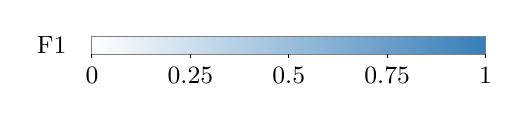
\begin{tikzpicture}[x=5cm,y=0.23cm,font=\small]
  \shade[left color=white,right color=classFOne] (0,0) rectangle (1,1);
  \draw[gray] (0,0) rectangle (1,1);
  \foreach \value in {0,0.25,0.5,0.75,1} {
    \draw (\value,0) -- (\value,-0.2);
    \node[anchor=north] at (\value,-0.2) {\value};
  }
  \node[anchor=east] at (-0.04,0.5) {F1};
\end{tikzpicture}
\endgroup

\caption[Four-class F1 by model configuration.]{Pooled four-class F1. Darker cells indicate higher scores on a common 0--1 scale; exact values are printed in each cell. Class supports are 1,103 anger, 1,636 happiness, 1,708 neutral, and 1,084 sadness.}
\label{fig:four-class-f1}
\end{figure}

Context's largest class gain was for sadness. Neutral remained the weakest class for both fusion variants, so their aggregate gains do not imply uniformly strong recognition.

\begin{table}[htbp]
\centering
\caption{Macro F1 by held-out session.}
\label{tab:session-fold-variation}
\small
\setlength{\tabcolsep}{5pt}
\begin{tabular}{|l|r|r|r|r|r|}
\hline
\textbf{Configuration} & \textbf{S1} & \textbf{S2} & \textbf{S3} & \textbf{S4} & \textbf{S5} \\ \hline
Utterance-only text & 0.6376 & 0.7125 & 0.6443 & 0.6575 & 0.6625 \\ \hline
Three-turn context & 0.6918 & 0.7556 & 0.7235 & 0.7310 & 0.7505 \\ \hline
Audio only & 0.6450 & 0.6974 & 0.5870 & 0.6017 & 0.6224 \\ \hline
Equal-weight fusion & 0.7517 & 0.8108 & 0.7708 & 0.8090 & 0.7922 \\ \hline
Validation-fitted fusion & 0.7294 & 0.8070 & 0.7542 & 0.7932 & 0.7852 \\ \hline
\end{tabular}
\end{table}

Table~\ref{tab:session-fold-variation} shows that context exceeded utterance-only text, and equal fusion ranked highest, in every session. Audio varied most. These five actor dyads show observed fold variation, not population-level speaker variability; unweighted fold means need not equal pooled scores.
